\documentclass[11pt, addpoints, answers]{exam}

\usepackage{amsmath, amssymb, amsthm, euler}
\usepackage{xcolor}
\usepackage{graphicx}
\usepackage{graphics}
\usepackage{tikz}
\usepackage{tikz-qtree}
\usetikzlibrary{graphs}
\tikzset{every tree node/.style={minimum width=2em,draw,circle},
    blank/.style={draw=none},
    edge from parent/.style=
    {draw,edge from parent path={(\tikzparentnode) -- (\tikzchildnode)}},
    level distance=1.2cm}
\usepackage{listings}   
\usepackage{caption}
\usepackage{algorithm}
\usepackage{algorithmicx}
\usepackage{algpseudocode}
\usepackage{underscore}
% \usepackage[top=2cm, bottom=2cm, left=2cm, right=2cm]{geometry}  
\makeatletter
\newcommand\dlmu[2][2.5cm]{\hskip1pt\underline{\hb@xt@ #1{\hss#2\hss}}\hskip3pt}
\makeatother

% For inserting code snippets.
\usepackage{listings}
\lstset{
    columns = fixed,
    basewidth = {0.5em},
    breaklines = true,
    backgroundcolor = \color{white},
    keywordstyle = \color[RGB]{40, 40, 255},
    numberstyle = \footnotesize\color{darkgray},
    commentstyle = \ttfamily\color{violet},
    basicstyle = \ttfamily,
    stringstyle = \ttfamily\color[RGB]{128, 0, 0},
    showstringspaces = false,
    language = {[11]C++},
    escapechar = \@
}
\lstnewenvironment{cpp}[1][]{\lstset{language = {[11]C++}, #1}}{}

\usepackage{tikz}

% headers, footers, titles
\newcommand{\CourseName}{CS101 Algorithms and Data Structures}
\newcommand{\HomeworkNO}{Homework 10}
\newcommand{\DueDate}{Due date: 23:59, December 4th, 2022}

\pagestyle{headandfoot}
\runningheadrule
\runningheader{\CourseName}{\HomeworkNO}{\DueDate}
\runningfooter{}{\thepage}{}

\title{
	\CourseName\\
	Fall 2022\\
	\HomeworkNO
}
\author{}
\date{\DueDate}

% formats of questions, choices, points, etc.
\qformat{\bf\thequestion. (\totalpoints\ points) \thequestiontitle\hfill}
\pointname{'}
\CorrectChoiceEmphasis{\bf\color{blue}}
\SolutionEmphasis{\color{blue}}

% We frequently use this font.
\newcommand{\ttt}{\texttt}

\begin{document}

\maketitle

\begin{enumerate}
	\item Please write your solutions in English.
	\item Submit your solutions to gradescope.com.
	\item Set your FULL name to your Chinese name and your STUDENT ID correctly in Account Settings.
	\item If you want to submit a handwritten version, scan it clearly. \ttt{CamScanner} is recommended.
	\item When submitting, match your solutions to the problems correctly.
	\item No late submission will be accepted.
	\item Violations to any of the above may result in zero points.
\end{enumerate}

\begin{questions}

\titledquestion{Multiple Choices}

Each question has \textbf{one or more}  answer(s). Select all the  answer(s). For each question, you will get 0 points if you select one or more wrong answers, but you will get 1 point if you select a non-empty subset of the  answers.

Write your answers in the following table.

%%%%%%%%%%%%%%%%%%%%%%%%%%%%%%%%%%%%%%%%%%%%%%%%%%%%%%%%%%%%%%%%%%%%%%%%%%%
% Note: The `LaTeX' way to answer a multiple-choices question is to replace `\choice'
% with `\Choice', as what you did in the previous questions. However, there are 
% still many students who would like to handwrite their homework. To make TA's work 
% easier, you have to fill your selected choices in the table below, no matter whether 
% you use LaTeX or not.
%%%%%%%%%%%%%%%%%%%%%%%%%%%%%%%%%%%%%%%%%%%%%%%%%%%%%%%%%%%%%%%%%%%%%%%%%%%

\begin{table}[htbp]
	\centering
	\begin{tabular}{|p{2cm}|p{2cm}|p{2cm}|p{2cm}|}
		\hline
		(a) & (b) & (c) & (d) \\
		\hline
		%%%%%%%%%%%%%%%%%%%%%%%%%%%%%%%%%%%%%%%%%%%%%%%%%%%%%%%%%%
		% YOUR ANSWER HERE.
		  AC  &  C  & C   & ABCD  \\
		%%%%%%%%%%%%%%%%%%%%%%%%%%%%%%%%%%%%%%%%%%%%%%%%%%%%%%%%%%
		\hline
	\end{tabular}
\end{table}

\begin{parts}
	\part[2] Which of the followings are true?  

	\begin{choices}
	    \CorrectChoice One Floyd-Warshall algorithm's step is to find $d^{(k)}_{i,j}$: that is, the shortest path allowing intermediate visits to vertices $v_1,v_2, ...,v_{k-1},v_k$.
		\choice Like Dijkstra's algorithm, Floyd-Warshall algorithm cannot work with any graph with negative weight edge.
        \CorrectChoice Floyd-Warshall algorithm can find the shortest path between all pairs of nodes while Dijkstra's algorithm is used to find single-source shortest path.
		\choice Floyd-Warshall algorithm uses greedy idea.
	\end{choices}
	
	\part[2] Which of the followings are true?  

	\begin{choices}
		\choice For A* graph search algorithm, it will always return an optimal solution if it exists.
		\choice For A* graph search algorithm with admissible heuristic, it will always return an optimal solution if it exists.
		\CorrectChoice For A* graph search algorithm with consistent heuristic, it will always return an optimal solution if it exists.
		\choice None of the above.
	\end{choices}
	
	\part[2] We run Floyd-Warshall algorithm on a graph with $n$ vertices $v_1,v_2,...,v_{n/2},..., v_n$ ($n$ is even). Suppose all three loops $(k, i, j)$ are iterated from $1$ to $n$. After running at least ______ iterations of the out-most loop $k$, it is ensured to find the shortest path between $v_{n/2}$ and $v_n$. 
		
	\begin{choices}
	    \choice $\frac{n}{2}-1$
	    \choice $\frac{n}{2}$
		\CorrectChoice $n-1$
		\choice $n$
	\end{choices}
	
	\part[2] Which of the following statements about shortest path algorithms is/are true?
	\begin{choices} 
	    \CorrectChoice If we modify the outer loop of Dijkstra’s algorithm to execute $|V|-1$ iterations instead of $|V|$ iterations (i.e. only pop $|V|-1$ times from the heap), the algorithm can still find the shortest path on a positive-weighted graph.
		\CorrectChoice We can modify Bellman-Ford algorithm to detect whether there exists a negative cycle or not in a directed graph.
		\CorrectChoice If we modify the outer loop of Bellman-Ford algorithm to execute $|V|$ iterations instead of $|V|-1$ iterations (i.e. apply update rule to each edge for $|V|$ times), the algorithm can still find the shortest path on a positive-weighted graph.
		\CorrectChoice We can modify Floyd-Warshall algorithm to detect whether there exists a negative cycle or not in a directed graph.
	\end{choices}
	
\end{parts}

\newpage

\titledquestion{Shortest Path}
\begin{parts}

\part[3] Consider the weighted undirected graph with $4$ vertices, where the weight of edge ${i, j}$ is given by the entry $W_{i,j}$ in the matrix $W$,
\begin{figure}[htbp]
    \centering
    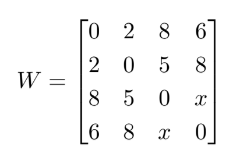
\includegraphics[width=0.2\linewidth]{fig/shortestPath.png}
\end{figure}

We want to find the largest possible integer value of $x$, for which at least one shortest path between some pairs of vertices will definitely contain the edge with weight $x$. What is this largest possible integer value of such $x$? Explain your reason briefly. When breaking tie, the path may be random.

\vspace{1in}



\part[4] Suppose $G = (V, E)$ is a weighted graph and $T$ is its shortest-path from source $s$ to $t$. If we increase all weights in $G$ by the same amount, i.e., $\forall e\in E$, $w'_e=w_e+c$. Is $T$ still the shortest-path from source $s$ to $t$ of the new graph? If yes, prove the statement. Otherwise, give a counter example.


\newpage

\titledquestion{A* algorithm}
Consider A* algorithm on the following graph. Edges are labeled with their costs, and heuristic values $h$ for nodes are labeled next to the nodes. $S$ is the start node, and $G$ is the goal node. Assume ties are broken in alphabetical order. Write your answer in the blank spaces provided.

\begin{figure}[htbp]
    \centering
    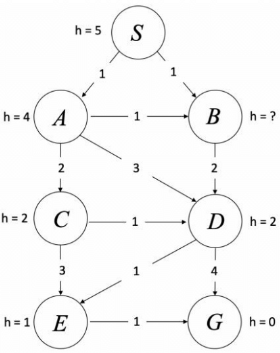
\includegraphics[width=0.3\linewidth]{fig/Astar.png}
\end{figure}

\begin{parts}
\part[3] With the heuristic values fixed for all nodes other than $B$, for which values of $h(B)$ will A* graph search be guaranteed to return the optimal path? (All heuristics are consistent.) Either fill in the lower and upper bound in the blank spaces below or write ``impossible” in two spaces.
$$\_\_\_\_ 4 \_\_\_\leq h(B)\leq \_\_\_ 4 \_\_\_\_$$

\part[3] Given the above heuristics, and choose (one of) the heuristic you answered in (a), write down the heuristic $h(B)$ you used. What is the order of the nodes that are going to be expanded in, assuming we run A* graph search on it.\\

$h(B)=\_\_\_ 4 \_\_\_$\\
Expand order:
%\vspace{1in}
\\$S,A,B,C,D,E,G$\\

\part[4] Based on (b), what path is returned?
\\$S,B,D,E,G$\\

\end{parts}


\newpage

\titledquestion{Floyd-Warshall algorithm}
\begin{parts}
    \part[4] Consider the following pseudo-code of the Floyd-Warshall algorithm. Assume $w_{ij}=\infty$ where there is no edge between vertex $i$ and vertex $j$, and assume $w_{ii}=0$ for every vertex $i$.
\begin{figure}[htbp]
    \centering
    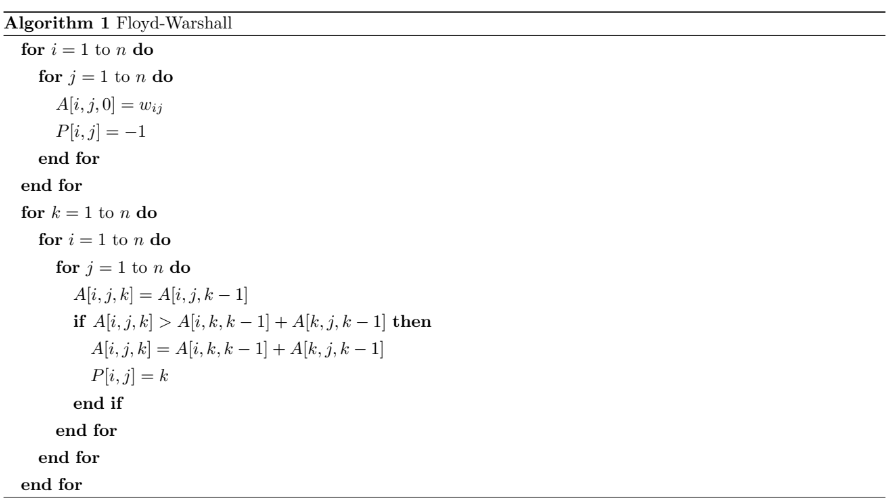
\includegraphics[width=1\linewidth]{fig/floyd-warshall.png}
\end{figure}
Assume matrix $P$, the output of the above algorithm, is given. Design an algorithm for finding the shortest path from $u$ to $v$ by using matrix $P$. You can show your algorithm with natural language or pseudo-code.
we can use the funcion $solution(u, v)$ to get the path from $u$ to $v$.
\begin{algorithm}[H]
    \begin{algorithmic}[1]
        \Function {solution}{$u$, $v$}
        \State path = []
        \If {$u == v$}
            \State path.push_back($u$)
            \State \Return path
        \EndIf
        \State path.push_back($u$)
        \State getpath($u, v, path$)
        \State path.push_back($v$)
        \State \Return path
        \EndFunction
    \end{algorithmic}
\end{algorithm}
to finish the getpath function above, we need to define a new function $getpath(u, v, path)$
\begin{algorithm}[H]
    \begin{algorithmic}[1]
        \Function {getpath}{$u, v, path$}
        \State $k = p[u, v]$
        \If {$k == -1$} 
            \State \Return 
        \EndIf
        \State getpath($u, k, path$)
        \State path.push_back($k$)
        \State getpath($k, v, path$)
        \EndFunction
    \end{algorithmic}
\end{algorithm}


\newpage

	\part[6] 
	Consider the following implementation of the Floyd-Warshall algorithm. Assume $w_{ij}=\infty$ where there is no edge between vertex $i$ and vertex $j$, and assume $w_{ii}=0$ for every vertex $i$. Add some codes in the blank lines to detect whether there is a \textbf{negative cycle} (the sum of weights of edges on the cycle is negative) in the graph. (You may not use all blank lines.)
\lstset{language=C}
\begin{lstlisting}    
bool detectNegCycle(int graph[][V]) 
{ 
    int dist[V][V], i, j, k; 
   
    for (i = 0; i < V; i++) 
        for (j = 0; j < V; j++) 
            dist[i][j] = graph[i][j]; 
   
    for (k = 0; k < V; k++) { 
        for (i = 0; i < V; i++) { 
            for (j = 0; j < V; j++) { 
                if (dist[i][k] + dist[k][j] < dist[i][j]) 
                        dist[i][j] = dist[i][k] + dist[k][j]; 
            } 
        } 
    } 
    
    for(i = 0; i < V; i++) {_____________
        if(dist[i][i] < 0) {_____________
            return true;_________________
        }________________________________
    }____________________________________
            
    return false;  
} 

\end{lstlisting}

\end{parts}
\newpage


\end{questions}

\end{document}